%!TEX program = xelatex
\documentclass[varwidth,border=0pt]{standalone}

% the various libraries we will be using
\usepackage{tikz}
\usetikzlibrary{calc}
\usepackage[none]{hyphenat}
\usepackage{lmodern}
\usepackage{fontspec}
\defaultfontfeatures{Ligatures=TeX}

% define colours
% taken from pickton on Adobe Kuler:
% https://kuler.adobe.com/Some-Kind-Of-Execushares-color-theme-3837185/
\definecolor{ExecusharesRed}{RGB}{230,37,52}
\definecolor{ExecusharesBlack}{RGB}{43,40,40}
\definecolor{ExecusharesBlue}{RGB}{22,190,207}
\definecolor{ExecusharesWhite}{RGB}{255,255,243}
\definecolor{ExecusharesGrey}{RGB}{107,110,108}

\usepackage{charter}
\DeclareMathVersion{mathchartertext}
\SetSymbolFont{letters}{mathchartertext}{OML}{mdbch}{m}{n}
\newcommand{\charmu}{\mathversion{mathchartertext}$\mu$\mathversion{normal}}

% use Adobe's Source Pro fonts:
% Source Serif Pro: http://store1.adobe.com/cfusion/store/html/index.cfm?store=OLS-US&event=displayFontPackage&code=1966
% Source Sans Pro: http://store1.adobe.com/cfusion/store/html/index.cfm?event=displayFontPackage&code=1959
% Source Code Pro: http://store1.adobe.com/cfusion/store/html/index.cfm?store=OLS-US&event=displayFontPackage&code=1960
\setmainfont{Source Serif Pro}
\setsansfont{Source Sans Pro}
\setmonofont{Source Code Pro}

\usepackage{amssymb}
\usepackage{amsmath}
\usepackage{pgfplots}
\pgfplotsset{compat=newest}
\usepackage{pgfplotstable}
\usetikzlibrary{plotmarks,arrows}
\usetikzlibrary{calc,patterns,decorations.pathmorphing,decorations.markings}
\tikzset{>=latex}
\usepackage{colortbl}

\begin{document}
	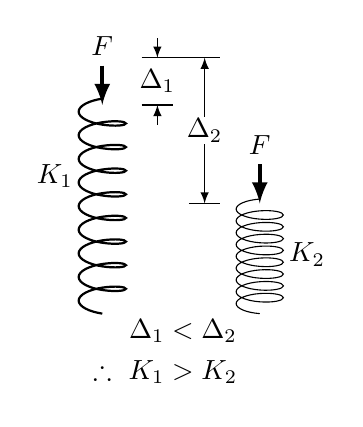
\begin{tikzpicture}
		\draw[decoration={aspect=0.3, segment length=3mm, amplitude=3mm,coil},decorate,thick] (0, 0) -- (0, 3);
		\draw[ultra thick,->] (0, 3.15) -- (0, 2.65);
		\node[anchor=east] at(-0.25, 1.75){$K_1$};
		\node[anchor=south] at(0, 3.15){$F$};

		\draw[decoration={aspect=0.3, segment length=1.5mm, amplitude=3mm,coil},decorate] (2, 0) -- (2, 1.5);
		\draw[ultra thick,->] (2,  1.9) -- (2,  1.4);
		\node[anchor=west] at(2.25,  0.75){$K_2$};
		\node[anchor=south] at(2,  1.9){$F$};

		\draw (0.5, 3.25) -- (1.5, 3.25);
		\node at (0.7, 2.95){$\Delta_1$};
		\draw (0.5, 2.65) -- (0.9, 2.65);
		\draw[->] (0.7, 3.5) -- (0.7, 3.25);
		\draw[->] (0.7, 2.4) -- (0.7, 2.65);

		\draw (1.1, 1.40) -- (1.5, 1.40);
		\node at (1.3, 2.325){$\Delta_2$};
		\draw[<-] (1.3, 3.25) -- (1.3, 2.5);
		\draw[->] (1.3, 2.150) -- (1.3, 1.40);

		\node[text width=2cm] at(0.8, -0.25){\begin{align*}\Delta_1 &< \Delta_2 \\ \therefore\ K_1 &> K_2\end{align*}};
	\end{tikzpicture}
\end{document}